\documentclass[10pt,conference]{IEEEtran}

% ---------------------------------------------------------------------------
% Execution-based conformance study of the MCP server ecosystem.
% Numeric macros in numbers.tex are AUTO-GENERATED by driver/make_numbers.py
% from the final dataset -- never hand-edit them; edit the analysis instead.
%
% MSR 2027 technical track build: IEEE conference template, double-anonymous.
% Limit is 10 pages of main text plus 2 pages that contain only references.
% ---------------------------------------------------------------------------

\usepackage[T1]{fontenc}   % T1: renders \_ and \{ in \texttt correctly and makes
                           % them extractable/searchable in the PDF (OT1 does not)
\usepackage{booktabs}
\usepackage{graphicx}
\usepackage{xcolor}
\usepackage{listings}
\usepackage{amsmath}
\usepackage{url}
\usepackage{hyperref}      % load last

\hypersetup{colorlinks=true, linkcolor=blue, citecolor=blue, urlcolor=blue,
            pdfauthor={}, pdfcreator={}, pdfproducer={}}

% AUTO-GENERATED by driver/make_numbers.py -- do not edit by hand.
\newcommand{\Nframe}{17,432}
\newcommand{\Nattempted}{6,106}
\newcommand{\NHarnessError}{17}
\newcommand{\Nprobed}{6,089}
\newcommand{\NEntrypointSeen}{466}
\newcommand{\NEntrypointUnreprobed}{4}
\newcommand{\HandshakeRateCl}{60.5\% (95\% CI 56.2--64.0)}
\newcommand{\ErrAsResultRateCl}{88.4\% (95\% CI 86.6--90.0)}
\newcommand{\NoTypecheckRateCl}{7.4\% (95\% CI 5.9--9.2)}
\newcommand{\MalformedDiesRateCl}{0.5\% (95\% CI 0.3--0.7)}
\newcommand{\GapRunnableCl}{16.1 pp (95\% CI 7.2--23.9)}
\newcommand{\GapErrAsResultCl}{-2.5 pp (95\% CI -6.0--1.6)}
\newcommand{\PctVerOffered}{97\%}
\newcommand{\NVerOffered}{3,576}
\newcommand{\NVerDowngraded}{104}
\newcommand{\NVerAhead}{5}
\newcommand{\TopPublisherHandshake}{26.2\%}
\newcommand{\TopPublisherDepressionPP}{1.8}
\newcommand{\HandshakeDesignEffect}{3.2}
\newcommand{\Nresponders}{3,685}
\newcommand{\HandshakeRate}{60.5\% (95\% CI 59.3--61.7)}
\newcommand{\HandshakeCount}{3685}
\newcommand{\ErrAsResultRate}{88.4\% (95\% CI 87.3--89.4)}
\newcommand{\ErrAsResultCount}{3258}
\newcommand{\NotErrAsResultPct}{11.6\%}
\newcommand{\UnknownProtoErrCount}{139}
\newcommand{\UnknownWrongCodeCount}{122}
\newcommand{\UnknownProseCount}{166}
\newcommand{\NoTypecheckRate}{7.4\% (95\% CI 6.6--8.3)}
\newcommand{\MalformedDiesRate}{0.5\% (95\% CI 0.3--0.7)}
\newcommand{\SilentExecTS}{112}
\newcommand{\SilentExecPy}{0}
\newcommand{\SilentExecTSvOne}{106}
\newcommand{\SilentExecTSCaret}{109}
\newcommand{\SilentExecTSExact}{0}
\newcommand{\Npublishers}{3,899}
\newcommand{\NuniqPub}{3,899}
\newcommand{\TopPublisherN}{305}
\newcommand{\TopPublisherPct}{5.0\%}
\newcommand{\TopTenPct}{12.6\%}
\newcommand{\HandshakeRatePub}{58.7\% (95\% CI 57.2--60.2)}
\newcommand{\ErrAsResultRatePub}{85.2\% (95\% CI 83.7--86.6)}
\newcommand{\NoTypecheckRatePub}{8.1\% (95\% CI 7.0--9.3)}
\newcommand{\NEntrypointBlocked}{462}
\newcommand{\EntrypointBlockedPct}{21.6\%}
\newcommand{\EntrypointRecovered}{44}
\newcommand{\EntrypointRecoveryRate}{9.5\% (95\% CI 7.2--12.5)}
\newcommand{\HandshakeCountCorr}{3,729}
\newcommand{\HandshakeRateCorr}{61.2\% (95\% CI 57.7--64.4)}
\newcommand{\HandshakeRateCorrBinom}{61.2\% (95\% CI 60.0--62.5)}
\newcommand{\NpmRate}{66.2\%}
\newcommand{\NpmN}{3,952}
\newcommand{\PypiN}{2,137}
\newcommand{\PypiRateRaw}{50.1\%}
\newcommand{\PypiRateCorr}{52.1\% (95\% CI 46.3--59.1)}
\newcommand{\GapRaw}{16.1}
\newcommand{\GapCorr}{14.0}
\newcommand{\NAcceptInvalid}{273}
\newcommand{\NSilentExec}{129}
\newcommand{\SilentExecShare}{47\%}
\newcommand{\SilentExecRate}{3.5\% (95\% CI 3.0--4.1)}
\newcommand{\NInBandError}{118}
\newcommand{\InBandShare}{43\%}
\newcommand{\NUnclassifiable}{26}
 % \Nframe, \Neligible, \Nprobed, \HandshakeRate, ... (generated)

% Anonymous artifact link for review (anonymous.4open.science mirror of the
% `artifact` branch). Restore the GitHub URL and add the Zenodo DOI for the
% camera-ready.
\newcommand{\ArtifactURL}{\url{https://anonymous.4open.science/r/mcp-conformance-F285}}

\title{Installed, Launched, Probed: An Execution-Based Conformance Census of the
Model Context Protocol Registry}

\author{\IEEEauthorblockN{Anonymous Author(s)}}

\begin{document}
\maketitle

\begin{abstract}
The Model Context Protocol (MCP) connects LLM agents to external tools, and public
registries now list tens of thousands of MCP servers. Most empirical studies of this ecosystem are \emph{static}: they scan
source code, mine issue trackers, or read registry metadata. None calls the tools of
registry servers at scale to check whether the servers start and follow the
protocol. This paper does. From the official registry (\Nframe{} unique servers) we
run a complete census of all \Nprobed{} self-contained, locally-installable servers.
Each is launched in an isolated sandbox and driven through a conformance harness that
checks the initialization lifecycle, tool listing and declared-schema validity, and
how the server handles an unknown tool name, a wrong-typed argument and a malformed
protocol frame. Only \HandshakeRateCorr{} of installable servers start and complete a
handshake. \ErrAsResultRate{} of responding servers report an unknown tool the same
way, which differs from the error reporting the specification illustrates. We trace
this to SDK defaults, and an open specification proposal would make it the specified
behavior. \SilentExecRate{} execute a tool on an argument their own declared schema
rejects and return a well-formed result that a client cannot tell apart from a correct
answer, although the specification requires servers to validate all tool inputs. Both
behaviors trace back to the SDKs, so they can be measured and fixed there. We release
the harness and the disclosure-filtered dataset.
\end{abstract}

\section{Introduction}
% - MCP's rise; registries at 17k+ servers; agents depend on these servers behaving.
% - The measurement gap: prior work is static (code scan / issue mining / metadata).
%   Analogy: the official conformance suite tests the 5 SDKs; nobody tests the
%   17,000 servers built on them.
% - A server can be "healthy" by maintenance metrics yet not start, or start yet
%   silently violate the protocol in ways that make agents fail confidently.
% - Contributions:
%   (C1) First execution-based, protocol-level conformance measurement of the MCP
%        ecosystem, at scale, fully reproducible.
%   (C2) A two-dimensional taxonomy: startup-failure classes and conformance-violation
%        classes, each tied to an agent-facing consequence.
%   (C3) Quantified spec-vs-practice divergence (error-as-result), traced to SDK defaults.
%   (C4) Open-source harness + released dataset.
Large language model agents increasingly act on the world through external tools,
and the Model Context Protocol (MCP) has become the dominant standard for
connecting them. In under two years MCP has gone from a single vendor's proposal
to an ecosystem with public registries listing tens of thousands of servers; the
official registry alone contains \Nframe{} unique servers at the time of our study.
When an agent selects a tool and an MCP server mishandles the request, by returning
a malformed result, accepting ill-typed arguments, or failing to start, the agent
does not merely lose a capability, and may proceed on wrong output with full
confidence. The reliability of this server layer is therefore a reliability
property of every agent built on top of it.

Yet we know remarkably little about how these servers actually behave, because most
published empirical studies of the MCP ecosystem examine servers \emph{without
running them}, and those that do run them look for vulnerabilities. Existing work scans source code and metadata for health and
maintainability, crawls registries to characterize scale and supply-chain
structure, or mines GitHub issues to taxonomize faults reported by users. These
static lenses answer valuable questions, but they cannot answer a prior and more
basic one: \emph{if you install these servers and speak the protocol to
them, do they work, and do they follow the specification?} The protocol maintainers
ship a conformance test suite, but it is built for SDK maintainers to run in
continuous integration, and to our knowledge it has not been used to measure the
deployed ecosystem. The SDKs are tested; the seventeen thousand servers built on them
are not.

This paper addresses that gap with an execution-based conformance study of the
MCP server ecosystem. Starting from the official registry, we execute a complete
census of every self-contained, locally-installable server, launch each in an
isolated sandbox, and drive it through a conformance harness that exercises the
initialization lifecycle, tool listing, declared-schema validity, and behavior
under three inputs that arise in ordinary agent sessions: a call to an unknown
tool, a call with a wrong-typed argument, and a malformed protocol frame. We grade
each server against the protocol version it negotiates, and we take care to
separate genuine specification requirements (RFC-2119 \textsf{MUST}/\textsf{SHOULD})
from behavior the specification merely illustrates by example.

Only \HandshakeRateCorr{} of installable servers start and complete a protocol
handshake. The rest fail in ways we classify into a startup-failure taxonomy, from
install errors to silent exits to hangs. Among servers that do respond,
\ErrAsResultRate{} report a call to a non-existent tool as a ``successful''
tool-execution error (\texttt{isError: true}) rather than the JSON-RPC protocol error
the specification illustrates. We trace this near-universal divergence to the default
behavior of the official SDKs, which is inherited by the servers built on
them. The result bears on a live debate, in which an open proposal would
reclassify unknown-tool failures to match what the SDKs already do, arguing the
change aligns the specification with practice~\cite{sep2145}. Our census says how far
practice has already gone, which decides whether such a change ratifies the ecosystem
or redirects it. Separately, \SilentExecRate{} of responding servers execute a tool on
an argument their own declared schema rejects and return a well-formed result. In one
case a code-scanning tool asked to scan an integer replied \texttt{CLEAN}, with
neither an error code nor an \texttt{isError} flag a client could act on. Unlike the
error-reporting question, this behaviour violates an explicit requirement that servers
validate all tool inputs. A further \MalformedDiesRate{} fail to recover from a malformed frame and
answer nothing further, although JSON-RPC 2.0 requires a reply to every request.

We organise the study around five research questions:

\begin{itemize}
  \item \textbf{RQ1 (Runnability).} What fraction of registry-published servers can a
    client install and start, and when they do not start, why not?
  \item \textbf{RQ2 (Lifecycle conformance).} Of the servers that respond, how many
    correctly implement the initialization lifecycle, tool listing, and declared-schema
    validity?
  \item \textbf{RQ3 (Input enforcement).} How many servers execute a tool on an
    argument their own declared schema rejects, and what does the client receive when
    they do?
  \item \textbf{RQ4 (Specification versus practice).} Where the specification and
    deployed behaviour disagree on error reporting, how large is the divergence, what
    causes it, and which side is moving?
  \item \textbf{RQ5 (Correlates).} Do runnability and conformance vary with the
    package registry a server ships on?
\end{itemize}

This paper makes four contributions:
\begin{itemize}
  \item \textbf{A protocol-level conformance measurement of the MCP ecosystem by
    execution} (C1): where prior ecosystem studies read code and metadata, we install
    and speak the protocol to a complete census of the eligible registry, testing
    behaviour against inputs rather than inspecting declarations, and releasing an
    open harness and dataset so the measurement is fully reproducible.
  \item \textbf{A two-dimensional taxonomy} (C2) of startup-failure classes and
    conformance-violation classes, each tied to a concrete agent-facing consequence.
  \item \textbf{A root-cause account of the spec--practice divergence} (C3): by
    attributing each server to its SDK, we show the dominant divergence is
    institutionalized in the official SDKs rather than independently reinvented.
  \item \textbf{Open infrastructure} (C4): a conformance harness that extends the
    official suite's scenarios to arbitrary deployed servers, plus the released
    measurement dataset, enabling the ecosystem to monitor its own conformance.
\end{itemize}


\section{Background and Related Work}
% - MCP protocol: stdio/JSON-RPC lifecycle, initialize/capabilities, tools/list,
%   tools/call, error semantics, protocol versioning.
% - Static ecosystem studies (code/metadata/issues): 1,899-server health study;
%   MCPCrawler 8,060-server measurement; runtime-fault taxonomies from GitHub issues.
% - Security-focused execution work (fixtures / curated vulnerable sets), and why
%   conformance is a distinct, unmeasured question.
% - Official conformance suite tests SDKs in CI, not the deployed ecosystem;
%   community discussion asking for a pre-publish conformance checklist.
\subsection{The Model Context Protocol}
MCP standardizes how LLM agents discover and invoke external tools. A client and
server negotiate a protocol version and capabilities during an \texttt{initialize}
handshake. The client can then list tools (\texttt{tools/list}) and invoke them
(\texttt{tools/call}). Messages follow JSON-RPC 2.0, including its error-object
semantics and its reserved error codes. Most deployments run the server locally over
stdio, where stdout carries protocol traffic and nothing else. The specification is
versioned by date, and servers may negotiate down to a version they support.

\subsection{Static studies of the MCP ecosystem}
The ecosystem has been studied at scale, but rarely by running it.
Health-and-maintainability work analyzes source and metadata for roughly 1,900
servers using static scanners and code-smell detectors~\cite{mcpfirstglance}, while
registry measurement crawls several marketplaces and characterizes scale,
maintenance and supply-chain concentration across some 8,000 servers from marketplace data, without running them~\cite{mcpcrawler}. A companion dataset effort catalogues 3,238 candidate MCP
repositories on GitHub and classifies them by operational role, again from repository evidence~\cite{mcpgithubdataset}, and a parallel line studies
the \emph{application} side, characterizing how 1,723 MCP applications configure and
supervise the servers they consume~\cite{mcpapps}. Fault taxonomies take a third
route and mine GitHub issues~\cite{runtimefaults,realfaults}. One finds tool faults
and data-schema faults the two most frequent categories~\cite{runtimefaults}, the same two areas our harness tests directly. None of this
work executes a server.

\subsection{Execution-based work is security-focused}
Some prior work does execute MCP servers, to find security problems. Sandboxed behavioral scanners hunt vulnerabilities in curated
corpora~\cite{sandboxscan}, taint-style analyzers confirm exploitable flaws across
tens of thousands of repositories~\cite{viper}, a security-invariants benchmark avoids live
third-party execution altogether in favor of fixtures and a 40-repository metadata
sample~\cite{securityinvariants}, and malicious-server detection, authentication
studies, and dynamic assessment of internet-facing endpoints scope to security
surfaces~\cite{maliciousmcp,remoteauth,exposedbydesign}.

MCPZoo assembles 64,611 unique servers, of
which more than 37,288 support dynamic analysis, and uses them to show that existing
security scanners are unreliable, with fewer than half of sampled alerts holding up
under manual validation~\cite{mcpzoo}. That corpus differs from ours in two ways. First, MCPZoo is built by \emph{repairing}
servers: a multi-agent framework infers environments and iteratively fixes deployment
and runtime defects so that in-the-wild repositories become running services. That
construction is the right choice for studying what a server does once it runs, and it
necessarily removes the signal we measure, which is how often a server runs at all
when a client installs it as published. Second, its population is collected from
multiple public markets, whereas ours is the official registry, the surface a client actually
resolves against. That their corpus needed a repair framework fits our runnability finding.
Conformance is a separate question: whether a server that is neither malicious nor vulnerable does what the
specification says.

Concurrently with our work, Afsar draws a seeded random sample of 400 npm stdio
servers from the same registry and probes each without repair: 48.8\% complete a
handshake, servers that never start (37.5\%) outnumber those missing credentials
(13.3\%), and the 195 that run show no fatal schema violations across 2,766
tools~\cite{randomdraw2026}. That study samples one package ecosystem and checks
declared structure. We census both npm and PyPI and test behavior, calling tools
with inputs the server should reject.

\subsection{The specification's own error-handling debate}
The categorization this paper measures is under active revision. SEP-1303, accepted
and reflected in the current specification, moved tool input validation errors out of
protocol errors and into tool execution errors, reasoning that a language model can
self-correct only from an error that reaches its context~\cite{sep1303}. SEP-2145,
open at the time of writing, extends the same treatment to tool resolution failures,
including unknown tools, and states its purpose as aligning the specification with
existing Python and TypeScript SDK behavior~\cite{sep2145}. We take no position on which mechanism is correct. We measure what
fraction of the deployed ecosystem the proposed alignment already describes.

Concurrent with this work, a practitioner census posted to the same proposal probed
roughly 10,500 \emph{remote} registry endpoints, harvested their tool lists, and
reported that \(88.8\%\) of mutating tools declare no output schema at all, arguing
that the proposal's output-validation clause is inert for most of the write
surface~\cite{siliroid2026census}. That measurement and ours are close to disjoint.
It probes hosted HTTP endpoints and reads declared metadata, whereas we install and
execute local stdio servers and test behavior against inputs. It addresses the
output-validation clause, and we address tool resolution and input enforcement.

\subsection{Conformance tooling and the gap we fill}
The protocol maintainers ship a conformance suite for testing client and server
implementations, built for SDK maintainers to run in continuous integration; to our
knowledge it has not been used to measure the deployed ecosystem. As far as we know, ours is the first reproducible conformance measurement of this ecosystem
that installs and executes the servers themselves and tests their behavior against
adversarial inputs, released with an open harness and dataset.


\section{Methodology}
We measure the MCP server ecosystem by \emph{executing} it. This section defines
the sampling frame, the conformance harness, the sandbox, and the grading rules
(Figure~\ref{fig:pipeline}). The harness and the released dataset make every number
reproducible.

\begin{figure*}[t]
  \centering
  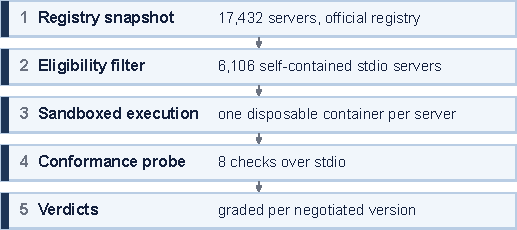
\includegraphics[width=0.85\textwidth]{figures/pipeline.pdf}
  \caption{Measurement pipeline. Every eligible server is installed and executed in
  its own disposable container, then driven through the conformance probe and graded
  against the protocol version it negotiates.}
  \label{fig:pipeline}
\end{figure*}

\subsection{Sampling frame}
We crawl the official MCP registry (\texttt{registry.modelcontextprotocol.io})
via its cursor-paginated API, retaining the latest published version of each
server. This yields \Nframe{} unique servers. Each server declares zero or more
\emph{packages} (installable artifacts on npm, PyPI, OCI, NuGet, or Cargo) and/or
\emph{remotes} (hosted HTTP endpoints). Our study population is the set of servers
that are (i) locally installable, (ii) use the \texttt{stdio} transport, (iii)
distributed on npm or PyPI (the two dominant registries), and (iv)
\emph{self-contained}: they declare no required environment variable or argument
that lacks a default. Criterion (iv) restricts us to servers that a client could
launch without provisioning secrets, which both bounds the ethics of mass
execution and defines a clean, reproducible population. We report the exclusion of
remote-only and credential-requiring servers explicitly (Section~\ref{sec:threats})
and treat the resulting frame as the denominator for all rates. We probe the
\emph{entire} frame (all \Nprobed{} eligible servers), so the measurement is a census of the eligible population.

\subsection{Conformance harness}
The harness, \texttt{mcpprobe}, is a deliberately minimal, hand-written JSON-RPC
client speaking line-delimited messages over the server's stdio. We do \emph{not}
use an official SDK client. To observe raw behavior, including responses to
malformed frames, the probe must not inherit any SDK-side correction or
validation. The harness offers protocol version \texttt{2025-06-18} at
initialization (the then-current revision was \texttt{2025-11-25}), records the
version the server \emph{negotiates}, and grades all later checks against that version. A server that supports the
offered version must answer with it, and \(3{,}576\) of \Nresponders{} responders did,
so almost all grading is against \texttt{2025-06-18}. Responding servers negotiated four distinct
revisions, and \(109\) of them settled on something other than the version we
offered, the oldest dating to 2024-11-05.

Each server is driven through the following checks, whose identifiers align with
the categories of the official \texttt{modelcontextprotocol/conformance} suite
where an analogue exists:

\begin{itemize}
  \item \textbf{server-initialize}: the \texttt{initialize} request must return a
    result carrying a protocol version and a capabilities object; the harness then
    sends \texttt{notifications/initialized}.
  \item \textbf{ping}: a \texttt{ping} must return an empty-object result.
  \item \textbf{tools-list}: if the server advertises the tools capability,
    \texttt{tools/list} must return an array in which every entry has a
    \texttt{name} and an \texttt{inputSchema} object.
  \item \textbf{tools-schema-valid}: each declared \texttt{inputSchema} must be a
    valid JSON Schema (checked by meta-validation).
  \item \textbf{tools-call-unknown}: calling a non-existent tool must be rejected.
    The specification's Error Handling section categorizes ``Unknown tools'' under
    \emph{Protocol Errors} (standard JSON-RPC errors) and illustrates this with a
    \texttt{-32602} example, as opposed to \emph{Tool Execution Errors} reported as
    a result with \texttt{isError: true}. This categorization is prose plus an
    example; it uses no RFC-2119 \textsf{MUST}/\textsf{SHOULD} keyword. We
    therefore do not treat a non-conforming response as a ``violation''; instead we
    record which of the two mechanisms the server uses (see
    \textsf{error-as-result} below).
  \item \textbf{tools-call-invalid-args}: for a tool with a typed required
    property, calling it with a wrong-typed value should be rejected. The spec is
    itself ambiguous here, since it lists ``Invalid arguments'' under Protocol Errors
    but ``Invalid input data'' under Tool Execution Errors, so we count \emph{either} a
    protocol error \emph{or} an \texttt{isError} result as acceptable, and flag only
    a plain success response (the tool ran on ill-typed input) as a defect.
  \item \textbf{malformed-json}: after receiving a syntactically invalid frame, the
    server must not crash or hang; a subsequent \texttt{ping} must still succeed.
  \item \textbf{stdout-purity}: under the stdio transport, the server must emit only
    protocol messages on stdout; any non-JSON line is a channel-corruption defect.
\end{itemize}

\subsection{Grading and the error-as-result category}
Verdicts are \textsf{pass}, \textsf{fail}, \textsf{warn}, \textsf{skip}, and one
category introduced by calibration: \textsf{error-as-result}. When validating the
harness against the official reference servers (\texttt{server-memory},
\texttt{server-everything}), we found they answer an unknown-tool call not with the
specified JSON-RPC \texttt{-32602} error but with a \emph{successful} response whose
\texttt{result.isError} flag is set. Because this behavior originates in the
official SDKs and is therefore ecosystem-wide, we grade it as its own category, not as a failure, and report its prevalence as a result.

\subsection{Sandbox}
Executing thousands of untrusted packages demands isolation. Each server runs in a
fresh container (\texttt{node:22-slim} for npm, an \texttt{astral-sh/uv} image for
PyPI) with a memory cap, a single CPU, a PID limit, \texttt{no-new-privileges}, all
Linux capabilities dropped, and no host filesystem mounts. The harness supports two
probe conditions. In the \textbf{two-phase}
condition, an online install pass populates the cache and the conformance probe then
runs with \texttt{-{}-network=none}, so no server code has network access while it is
being measured. In the \textbf{single-phase} condition, install and probe occur
together in one ephemeral container and the network is available throughout. The
census reported here was measured in the single-phase condition, for the operational
reasons given in Section~\ref{sec:method-env}, and we state the consequences for
validity in Section~\ref{sec:threats}.

\subsection{Execution environment and probe condition}
\label{sec:method-env}
The census was executed on a single disposable cloud instance (no cloud
credentials attached, so the blast radius of running untrusted code is one
throwaway host) using the online single-phase condition: install and probe occur
in one ephemeral \texttt{-{}-rm} container per server, with nothing cached between
servers so that disk usage stays bounded across the full ecosystem; the recorded
launch command of every run confirms that no volume was mounted. We did not run a
controlled comparison of the two conditions. In development runs on smaller subsets,
error-as-result prevalence (\(87\%\)) and silent type non-enforcement (\(7\%\)) among
responding servers were the same under both conditions; handshake yields from those
runs are not comparable, because the subsets differed. Two groups of runs ended for
reasons outside the server's control or of uncertain cause: \(32\) probes
(\(0.5\%\)) were killed (exit 137) by either the memory cap or an automated guard
that reclaims host disk space, and the census does not record which; \(17\) probes
(\(0.3\%\)) aborted on a harness-side error before any check ran. All but one of
these \(49\) are counted as non-handshaking, so they can only lower the handshake
yield; the exception was killed after completing its handshake.

\subsection{SDK-level confirmation}
\label{sec:sdk-probe}
Where a conformance failure concentrates in one SDK family, the census alone cannot
say whether the library permits the failure or the authors introduced it
independently. For the input-validation result we tested the SDK directly. We build two minimal servers exposing one tool that declares a
single required string property, one using the low-level \texttt{Server} API and one
using the high-level \texttt{McpServer} API, both on the same SDK release, and drive
each with the same harness check used in the census: a \texttt{tools/call} carrying an
integer where the declared schema requires a string. The construction is otherwise
identical, so any difference in outcome is a property of the API path. We report the
result in Section~\ref{sec:consequences}. The two servers and the probe script are
released with the harness.

\subsection{Funnel accounting}
Because ``does it even run'' is itself a research question, we count every stage:
declared $\rightarrow$ eligible (self-contained stdio npm/PyPI) $\rightarrow$
container started $\rightarrow$ process launched
$\rightarrow$ handshake completed $\rightarrow$ probed. Servers that never reach a
handshake are classified into startup-failure categories
(Section~\ref{sec:results}) from their exit code and stderr, so that the lost yield can be explained.


\section{Results}
\label{sec:results}

We launched all \Nattempted{} servers in the eligible frame. On \NHarnessError{} of
them the harness itself failed, through a broken pipe or an uncaught exception in our
probe, and those runs carry no verdict about the server. We report them here and
exclude them from every denominator, leaving \Nprobed{} graded servers.

\subsection{RQ1: Runnability and the startup funnel}
\HandshakeCountCorr{} of \Nprobed{} servers (\HandshakeRateCorr{}) complete the MCP
handshake once the entry-point artifact described in Section~\ref{sec:rq5} is
corrected; the uncorrected census figure is \HandshakeRate{}. Roughly two in five
never serve the protocol. Figure~\ref{fig:failures} classifies those failures
by cause.

Servers that only need credentials or configuration are counted apart from servers
that crash, since a missing setting is a documentation gap. Most failures happen
\emph{after} a successful install: the package downloads, then the process crashes,
hangs, or exits without speaking the protocol. The software fails after the packaging
has done its job. A concurrent random draw of 400 npm
servers reports a 48.8\% handshake rate~\cite{randomdraw2026}, against \NpmRate{} for
the npm servers in our census. Snapshot and harness both differ between the two
studies, which is enough to explain a gap of that size.

\begin{figure}[t]
  \centering
  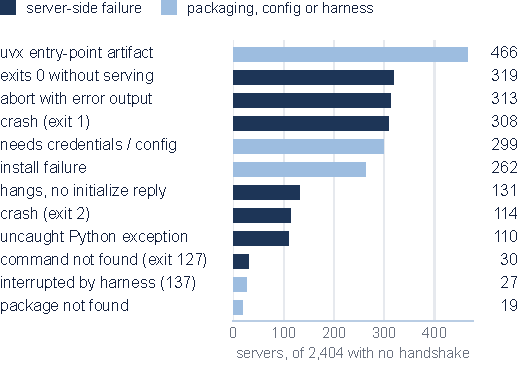
\includegraphics[width=\linewidth]{figures/failures.pdf}
  \caption{Why servers never reach a handshake. Configuration requirements and the
  entry-point artifact are separated from genuine startup failures.}
  \label{fig:failures}
\end{figure}

\begin{table}[t]
\centering
\caption{Startup-failure taxonomy: causes for servers that never reach a handshake.}
\label{tab:startup}
\begin{tabular}{lrr}
\toprule
Failure class & Count & \% of failures \\
\midrule
entrypoint-not-provided & 466 & 19.4 \\
exit-silent & 319 & 13.3 \\
crash-with-error-output & 313 & 13.0 \\
crash-exit-1 & 308 & 12.8 \\
needs-auth-or-config & 299 & 12.4 \\
install-error & 262 & 10.9 \\
hang-no-reply & 131 & 5.4 \\
crash-exit-2 & 114 & 4.7 \\
crash-python-exception & 110 & 4.6 \\
crash-exit-127 & 30 & 1.2 \\
crash-exit-137 & 27 & 1.1 \\
install-not-found & 19 & 0.8 \\
unclassified & 2 & 0.1 \\
crash-exit-255 & 1 & 0.0 \\
crash-exit-3 & 1 & 0.0 \\
crash-exit-4 & 1 & 0.0 \\
crash-exit-254 & 1 & 0.0 \\
\midrule
Total non-handshaking & 2404 & 100.0 \\
\bottomrule
\end{tabular}
\end{table}

\subsection{RQ2--RQ3: Conformance and robustness}
Table~\ref{tab:verdicts} reports the verdict distribution for each check over the
\Nresponders{} responding servers, with 95\% Wilson confidence intervals. Lifecycle
and tool-listing conformance are high, and the discriminating checks are error handling,
argument type enforcement, and malformed-input survival. \NoTypecheckRate{} of
responders failed to reject a wrong-typed required argument, which
Section~\ref{sec:consequences} decomposes into the servers that reported the problem
anyway and the smaller class that did not. \MalformedDiesRate{} failed to recover from a
malformed frame. We classify that as a robustness and conformance failure. The
security reading does not survive the transport: under stdio the client is the parent
process and the sole writer to the server's standard input, and a party able to
deliver a malformed frame can already terminate the subprocess. JSON-RPC 2.0, on which MCP is built,
nonetheless defines a parse-error response for this case and requires a reply to
every subsequent request~\cite{jsonrpc}, and these servers give neither. One
maintainer who reproduced the finding made this argument, and the classification here
follows it (Section~\ref{sec:threats}).

\begin{table}[t]
\centering
\caption{Verdict distribution per check over responding servers, with 95\% Wilson CIs on the pass (or documented) rate.}
\label{tab:verdicts}
\begin{tabular}{lrrrr}
\toprule
Check & Pass & Fail & Other & Pass rate (95\% CI) \\
\midrule
server-initialize & 217 & 0 & 0 & 100.0 (98.3--100.0) \\
ping & 216 & 1 & 0 & 99.5 (97.4--99.9) \\
tools-list & 215 & 2 & 0 & 99.1 (96.7--99.7) \\
tools-schema-valid & 214 & 1 & 0 & 98.6 (96.0--99.5) \\
tools-call-unknown & 7 & 12 & 198 & 3.2 (1.6--6.5) \\
tools-call-invalid-args & 197 & 15 & 5 & 90.8 (86.2--94.0) \\
malformed-json & 215 & 2 & 0 & 99.1 (96.7--99.7) \\
stdout-purity & 217 & 0 & 0 & 100.0 (98.3--100.0) \\
\bottomrule
\end{tabular}
\end{table}

\subsection{RQ3 refined: what a failure to reject actually returns}
\label{sec:consequences}
The \texttt{tools-call-invalid-args} verdict records whether a server rejects an
argument that violates its own declared schema. As a protocol judgment that
is correct, but it cannot tell a client what it received, because two different
behaviors produce the same verdict. A server may validate the input and
report the problem in the result \emph{text} without setting \texttt{isError}, which
is non-conformant but leaves the information available. Or it may execute the tool
and return ordinary-looking output, which does not. We separate the two by
classifying the recorded response of every server in this category
(Figure~\ref{fig:consequences}, Table~\ref{tab:consequences}).

\begin{figure}[t]
  \centering
  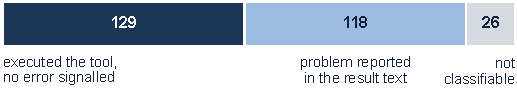
\includegraphics[width=\linewidth]{figures/consequences.pdf}
  \caption{The coarse verdict splits in half. Only the left segment is undetectable
  by the client: the tool ran on input its schema rejects and returned a well-formed
  result carrying no error indication.}
  \label{fig:consequences}
\end{figure}

Of \NAcceptInvalid{} such servers, \NInBandError{} (\InBandShare{}) reported the
problem in the result text, so the server noticed and a client willing to parse prose
could too. \NSilentExec{} (\SilentExecShare{}) executed the tool and returned a
result with no indication that anything was wrong. For \NUnclassifiable{} the
response could not be classified from the transcript. The hazard class is therefore \SilentExecRate{} of responding servers, smaller than the \NoTypecheckRate{} of the raw verdict, and it is the figure we report. We
count a server as reporting the problem whenever its output contains any error-like
token, so \NSilentExec{} is a lower bound.

This is not a matter of interpretation. The
specification's security requirements state that servers \textbf{MUST} validate all
tool inputs~\cite{mcpspec}. A server that executes a tool on an argument contradicting
its own published schema has not validated that input, so these \NSilentExec{} servers
fail an explicit RFC-2119 requirement, as do the servers that write non-protocol output to stdout, which the stdio transport forbids with a \textsf{MUST NOT}.

Here SDK attribution narrows the cause further than it does for the
error-reporting divergence. \SilentExecTS{} of the \NSilentExec{} are built on
the official TypeScript SDK and \SilentExecPy{} on either Python SDK, against
responding populations of \SDKPopTS{} and \SDKPopPy{} respectively. A behavior absent from one
language ecosystem and concentrated in another points to the library, so we tested the SDKs directly (Section~\ref{sec:sdk-probe}). On
\texttt{@modelcontextprotocol/sdk} 1.30.0, the current release at the time of writing,
a server built with the low-level \texttt{Server} API publishes an
\texttt{inputSchema} in \texttt{tools/list} and the SDK then does not check
\texttt{tools/call} arguments against it: a tool declaring a string property, called
with an integer, runs and returns a well-formed result. The same tool built with the
high-level \texttt{McpServer} API, whose schemas carry type information the SDK
already validates, rejects the identical call with an \texttt{isError} result. We did
not test the Python SDKs under the same conditions, so we report their absence from this population as an observation only. Within
the TypeScript SDK the gap is that one supported construction path publishes a
contract the library never enforces, so the servers on it have not declined a check
the SDK offered them. Of the \SilentExecTS{} TypeScript-SDK servers,
\SilentExecTSCaret{} declare a caret range and none declares an exact version.
Because each server was installed fresh, those ranges resolve to the newest 1.x, so this is current behavior, and a fix on the 1.x line
would reach almost all of them at their next install.

The unknown-tool divergence has a merged fix that deployed servers do not show. The
SDK's tracker records tool resolution as corrected in March 2026, four months before
our crawl, by a change that moves the tool-not-found check outside the handler's
\texttt{try} block so it propagates as a protocol error~\cite{sdkpr1389,sdkissue1510}.
We rebuilt the minimal high-level server on releases 1.28.0, 1.29.0 and 1.30.1 and
sent the same unknown-tool call. All three answer with an \texttt{isError} result
whose text reads \texttt{MCP error -32602: Tool \ldots{} not found}. The protocol
error is raised and then delivered inside a successful response, where a client
branching on JSON-RPC errors cannot see it. This explains a puzzle in our own data:
the census ran after the fix shipped, and the rate did not move.

The low-level path loses the tool name as well, which we had not tested. That API
takes one handler for every \texttt{tools/call} request, and the handler receives the
requested name without the library checking it against the declared tool list. Our
probe asked a low-level server for a tool it does not have and received that server's
ordinary answer, reporting a clean scan of code it was never given. Nothing in the
response marks the tool as missing.

In the recorded responses, a code-scanning tool asked to
scan the integer \texttt{12345} answered \texttt{CLEAN}, a prompt-scoring tool returned
a complete rubric including per-dimension sub-scores for the same integer, and a project
registry confirmed that a project named \texttt{12345} had been registered. All three are well-formed successful results. None relates to the question asked,
and at the protocol level none can be told apart from a correct answer: there is no
error code and no \texttt{isError} flag. Each server published a schema that would
have caught the call and then left it unenforced.

\begin{table}[t]
\centering
\caption{Servers that executed a tool on an argument their own declared schema
rejects, and returned ordinary-looking output. Inputs are the harness's type-poisoned
values; outputs are verbatim, truncated. None carries an error indication a client
could act on.}
\label{tab:consequences}
\small
\begin{tabular}{p{0.30\linewidth}p{0.20\linewidth}p{0.42\linewidth}}
\toprule
Tool & Argument sent & Result returned to the client \\
\midrule
\texttt{scan\_code\_imports} & \texttt{code: 12345} &
``CLEAN --- No npm package imports found in the provided code'' \\
\addlinespace
\texttt{register\_project} & \texttt{name: 12345} &
``Project 12345 registered successfully. Framework: generic'' \\
\addlinespace
\texttt{score\_prompt} & \texttt{prompt: 12345} &
a complete scoring rubric: \texttt{score: 8}, \texttt{grade: "F"}, with per-dimension
sub-scores \\
\addlinespace
\texttt{upcoming\_deadlines} & \texttt{within\_days: "not-a-number"} &
a dated regulatory snapshot with a populated result envelope \\
\addlinespace
\texttt{search} & \texttt{query: 12345} &
\texttt{\{"results":[]\}} \\
\bottomrule
\end{tabular}
\end{table}


\subsection{RQ4: Where practice and specification disagree, and which one moved}
\ErrAsResultRate{} of responding servers reported a call to a non-existent tool as an
\texttt{isError} tool-execution result instead of a JSON-RPC protocol error. The
specification's error-handling section lists ``unknown tool'' under \emph{Protocol
Errors} and illustrates it with a \texttt{-32602} example~\cite{mcpspec}. It attaches
no RFC-2119 keyword. We record which mechanism each server uses and score neither
as a violation (Section~\ref{sec:threats}).

The specification has been moving toward what servers do. SEP-1303, now
accepted and reflected in the specification, reclassified input validation errors from
protocol errors to tool execution errors on the grounds that a model can only
self-correct from an error it can see~\cite{sep1303}. SEP-2145, open at the time of
writing, proposes the same move for tool resolution failures, covering unknown and
disabled tools, and gives as its rationale that it ``aligns specification with existing
Python and TypeScript SDK behavior''~\cite{sep2145}. Our census measures how much of
the deployed ecosystem that alignment already describes: \ErrAsResultRate{} of
responding servers. (Aggregate figures from this census were posted to the
proposal's discussion thread while it was open.) The other \NotErrAsResultPct{} are
not one population: \UnknownProtoErrCount{} servers emit a protocol error coded
\texttt{-32602} or \texttt{-32601}, \UnknownWrongCodeCount{} use some other code, and
\UnknownProseCount{} return a plain success that states the failure only in its text,
a mechanism neither proposal describes.

To explain the uniformity, we attribute each server to its SDK from its resolved
dependency graph (Figure~\ref{fig:sdk}, Table~\ref{tab:sdk}). We take the exact
package version the probe launched and resolve its runtime dependencies through
deps.dev, so a server that reaches an SDK through a third-party wrapper is credited
to that SDK and not to the residual. \SDKDirect{} servers depend on an SDK directly
and \SDKIndirect{} reach one only through a wrapper. For \SDKUnattributed{} we have
no graph: the package or the probed version has since been withdrawn from its
registry. The behavior tracks the SDK: the
official TypeScript and Python SDKs and the FastMCP framework all default to it. A
small number of TypeScript-SDK servers emit the protocol error, so the alternative is
reachable within the SDK and simply is not the default. The official reference servers
behave the same way.

Our attribution recognizes a fixed list of known SDK package names, so the residual
\textsf{no-known-SDK} category holds servers with none of those names anywhere in
their runtime graph. Such a server may still have vendored an SDK at build time.
Resolving the graph transitively moves servers that inherit an SDK through a wrapper
into that SDK's family. That leaves the residual as the sharpest contrast in the
table: \SDKNoSDKRate{} of its \SDKNoSDK{} servers answer an unknown tool with an
\texttt{isError} result, against about nine in ten in every official-SDK family.
A few SDK defaults, used directly or through wrappers, account for this behavior
across the ecosystem. Where they are absent, so is the behavior.

\begin{figure}[t]
  \centering
  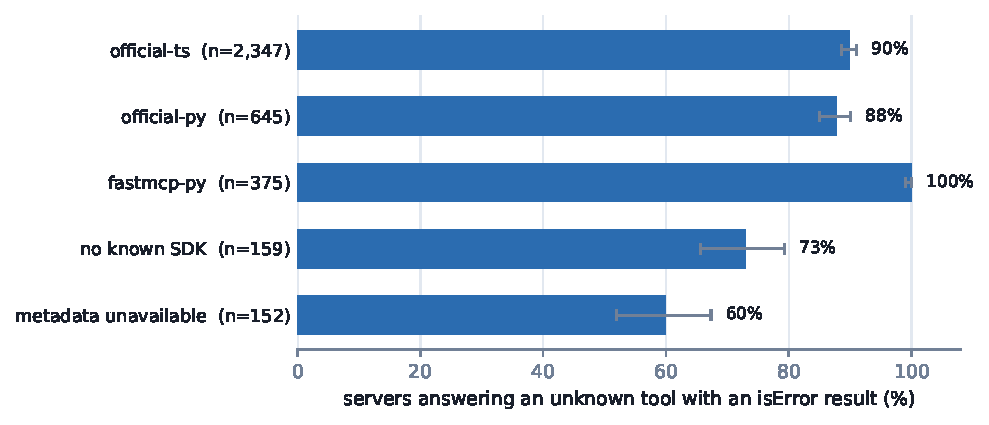
\includegraphics[width=\linewidth]{figures/sdk.pdf}
  \caption{Unknown-tool responses by SDK family. In every family, most servers answer with an \texttt{isError} result. Bars show 95\% Wilson intervals;
  families with fewer than 25 servers appear in Table~\ref{tab:sdk} only.}
  \label{fig:sdk}
\end{figure}

\begin{table}[t]
\centering
\caption{SDK family vs.\ unknown-tool response. Which mechanism a server uses tracks the SDK it was built on, not the author.}
\label{tab:sdk}
\begin{tabular}{lrrr}
\toprule
SDK family & error-as-result & protocol error & other \\
\midrule
official-ts & 2211 & 65 & 173 \\
official-py & 567 & 0 & 82 \\
fastmcp-py & 378 & 0 & 0 \\
no-known-SDK & 86 & 63 & 33 \\
metadata-unavailable & 16 & 2 & 0 \\
fastmcp-ts & 0 & 8 & 0 \\
xmcp-ts & 0 & 1 & 0 \\
\bottomrule
\end{tabular}
\end{table}

\subsection{RQ5: Correlates}
\label{sec:rq5}
We test whether runnability and conformance correlate with the package registry
(Figure~\ref{fig:byregistry}). Runnability differs: npm servers complete a
handshake far more often than PyPI servers (\NpmRate{} of \NpmN{} against
\PypiRateRaw{} of \PypiN{}, a difference of \GapRunnableCl{}). Conformance does not:
the same publisher-cluster bootstrap puts the error-as-result difference at
\GapErrAsResultCl{}, an interval spanning zero. We apply one method to both
comparisons so that neither rests on a stronger footing. The pattern follows from RQ4: because the
divergence is inherited from the SDKs, and both language ecosystems' SDKs share the
same default, the registry a server ships on changes whether it \emph{starts} but not
whether it \emph{conforms}.

Part of this gap came from our own launcher, and we corrected for it. We launch PyPI servers as \texttt{uvx <package>}, which resolves only
if the package's console script is named after the package; npm's \texttt{npx}
resolves the entry point from \texttt{package.json} and has no such requirement.
\NEntrypointBlocked{} PyPI servers (\EntrypointBlockedPct{} of the PyPI population)
installed successfully but were never launched for this reason alone. Our classifier
identifies \NEntrypointSeen{} such rows in the census; the completed re-probe covers
\NEntrypointBlocked{} of them, and \NEntrypointUnreprobed{} were missed. We
re-probed those servers with the entry point resolved from the installed package
metadata. \EntrypointRecovered{} (\EntrypointRecoveryRate{}) then completed a
handshake; the rest failed for reasons unrelated to naming (Python exceptions, hangs,
undeclared configuration). Correcting for this raises PyPI runnability from
\PypiRateRaw{} to \PypiRateCorr{} and the overall census figure to
\HandshakeRateCorr{}, which we report as the headline throughout. The npm--PyPI gap
narrows from \GapRaw{} to \GapCorr{} percentage points but stays large.

The entry-point problem is itself an ecosystem finding. Registry metadata does not
record a server's entry point, so a client following the registry alone cannot launch
a fifth of published PyPI servers, and once the entry point is resolved, nine in ten
of those servers still fail to start. A listing in the registry says
nothing about either.

\begin{figure}[t]
  \centering
  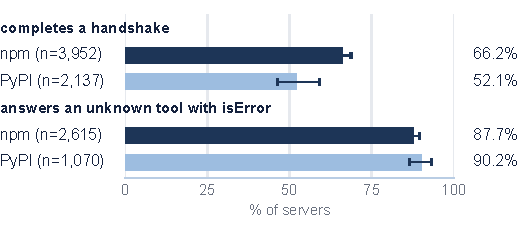
\includegraphics[width=\linewidth]{figures/by_registry.pdf}
  \caption{Handshake yield (PyPI after the entry-point correction) and the
  error-as-result rate for unknown tools, by package registry, with 95\% intervals
  from a publisher-cluster bootstrap.}
  \label{fig:byregistry}
\end{figure}


\section{Discussion}
% - Why the divergence exists (SDK monoculture) and what it means for agents.
% - Startup failure as an availability tax on agent pipelines.
% - Implications for the registry (pre-publish conformance gate) and SDK defaults.
\paragraph{The specification and the SDKs}
SEP-1303 moved input validation errors from protocol errors to tool execution errors,
arguing that a model can only correct an error it sees~\cite{sep1303}. SEP-2145
proposes the same change for unknown tools, so that the specification matches what
the SDKs already do~\cite{sep2145}. Our census shows how far that behavior has
spread: \ErrAsResultRate{} of responding servers. If SEP-2145 is adopted, it will
mostly describe what servers already do, and the servers that would have to change
are the minority that follow the current text.

\paragraph{Measuring at the SDK level}
Once servers are attributed to their SDKs, what looked like thousands of separate
decisions reduces to a few library defaults, some of them passed on again through
third-party wrappers. Changing a few SDKs would change most of the
population, so monitoring conformance should start with the SDKs.

\paragraph{Input validation}
The unknown-tool question is contested, and we do not score it. Input validation is
different. The specification requires servers to validate all tool inputs, yet
\NSilentExec{} servers run tools on arguments that their own schemas reject and return
results with no sign of a problem. No pending proposal would relax this requirement,
and a client cannot recover the missing information afterwards. Nothing in the
registry, the package metadata, or a static scan shows which servers enforce their
schemas; only running them does.

\paragraph{Startup failure}
Two in five installable servers never serve the protocol, and a fifth of PyPI servers
cannot be launched from registry metadata alone, because the metadata does not record
an entry point. The registry does not say whether a server starts. A pre-publish
check, which our harness can perform, would give clients that information.

\paragraph{Recommendations}
For the specification: decide SEP-2145 with these numbers available. For SDK authors:
validate declared argument types before dispatch by default, which would close a gap that violates an explicit MCP requirement. For agent frameworks:
validate arguments against the declared schema on the client side, because
\SilentExecRate{} of responding servers do not, and nothing in their responses shows it.


\section{Threats to Validity}
% - Construct: harness judges vs negotiated version; error-as-result graded as a
%   distinct category, not a fail. Internal: sandbox heterogeneity, offline condition.
% - External: sampling frame is self-contained stdio npm/PyPI servers; remote-only
%   and key-requiring servers excluded (enumerated). Reproducibility: pinned versions.
\label{sec:threats}

\paragraph{Construct validity}
Our verdicts operationalize ``conformance,'' and a poorly chosen operationalization
could over- or under-count. Three choices limit that risk. Our checks cover
requirements that every revision in the census states in the same terms, which keeps
any server from being judged against a rule that postdates the revision it
negotiated. We also distinguish normative requirements from illustrative
ones, and the most prevalent divergence we report (unknown-tool responses) is graded as
a distinct \textsf{error-as-result} category, not as a failure, because the specification expresses it only in prose and an example, without an RFC-2119 keyword. Third, we calibrated the harness against the official reference
servers before the study and confirmed it reproduces their known-good behavior on
every check except the SDK-level divergence we set out to measure.

\paragraph{Internal validity}
The census was measured in the single-phase condition, with the network available
during both install and probe (Section~\ref{sec:method-env}). This avoids penalizing
a server that legitimately contacts the network during initialization, but it does
not remove server-side outbound calls as a confounder. The exposure is concentrated
in one check. For \textsf{tools-call-invalid-args} we accept an \texttt{isError}
result as evidence that the server rejected the ill-typed argument; an
\texttt{isError} produced instead by an unrelated runtime or network failure is
indistinguishable to the harness, and would be counted as argument checking that did
not in fact occur. The reported rate of silent type non-enforcement is therefore a
\emph{lower bound}. The lifecycle, tool-listing, error-handling, malformed-input and
stdout-purity checks are local protocol behaviors and are not exposed to this
confound. A network-isolated replication would tighten the argument-checking result,
and the harness supports that condition directly. Sandbox heterogeneity across
language runtimes is a further
source of noise, which we bound by launching each package at the version its registry
entry declares and recording every run's full launch command, including the
base-image tag.

\paragraph{External validity}
Our population is self-contained, locally-installable servers distributed on npm and
PyPI using the stdio transport. This excludes remote-only servers (which we cannot
execute without provisioning hosted infrastructure) and servers requiring
credentials (which we exclude for both ethics and reproducibility). We report the
size of each excluded class explicitly and confine all rates to the stated frame;
we do not claim they generalize to remote or credentialed servers, whose conformance
is important future work. Agent clients mostly launch local stdio servers, which is why we studied this
population first.

\paragraph{Completeness}
Because we census the eligible frame, the counts are population counts. The intervals
we report do not describe sampling error. They describe how far a rate would move if
the registry had drawn a different set of publishers, which is the uncertainty that
matters when a single publisher ships hundreds of servers from one template.

\paragraph{Publisher clustering}
The \Nprobed{} servers in our frame come from only \Npublishers{} distinct registry
namespaces, and the distribution is heavy-tailed: the largest single publisher
accounts for \TopPublisherN{} servers (\TopPublisherPct{} of the census) and the ten
largest for \TopTenPct{}. Servers from one publisher frequently share a template and
behave near-identically, so a binomial interval that treats them as independent trials
is too narrow. Every interval in this paper therefore comes from a bootstrap that
resamples publishers instead of servers. The widening is substantial: the handshake
interval is \HandshakeDesignEffect{} times wider than the binomial one
(\HandshakeRateCl{} against \HandshakeRate{}). Error-as-result becomes
\ErrAsResultRateCl{} and silent type non-enforcement \NoTypecheckRateCl{}. As a second
check we recompute each rate on a subset holding one server per namespace
(\NuniqPub{} servers): handshake yield \HandshakeRatePub{}, error-as-result
\ErrAsResultRatePub{}, silent type non-enforcement \NoTypecheckRatePub{}. No
conclusion changes under either treatment. The largest publisher is atypical in
runnability, at a \TopPublisherHandshake{} handshake yield, and its presence moves the
census figure by \TopPublisherDepressionPP{} percentage points.

\paragraph{Severity of the malformed-frame finding, and a limitation it exposed}
We initially characterized failure to recover from a malformed frame as a
denial-of-service primitive. A maintainer who reproduced the finding independently
argued that this overstates it. The argument holds. Under the stdio transport the client
launches the server and is the sole writer to its standard input, so a party capable of
sending a malformed frame can already terminate the subprocess; the specification also
places the obligation not to send invalid messages on the client. The correct reading
is a robustness and conformance failure, and this paper reports it that way. The same maintainer traced the
behavior in their server to the official Go SDK's stdio transport, so this check,
like the unknown-tool divergence, can measure an SDK default that the server only inherits.

Another maintainer's fix exposed a limitation in our instrument. In their server the
process stayed alive while its parser absorbed the frames that followed, so the next
\texttt{ping} timed out. Our harness records a single verdict for
``did not answer after a malformed frame'' and does not distinguish a terminated
process from a desynchronized one. Both are conformance failures, but they are
different failures with different fixes, and \MalformedDiesRate{} therefore aggregates
the two. Separating them requires per-server process-state tracking that the released
transcripts support but the current verdict does not encode.

\paragraph{Interrupted probes}
\(49\) probes (\(0.8\%\)) ended for reasons that may lie outside the server
(Section~\ref{sec:method-env}): \(32\) killed by the memory cap or the disk guard, and
\(17\) aborted by a harness-side error. Counting \(48\) of them as non-handshaking can
depress the handshake yield by at most \(0.8\) percentage points and does not affect
conformance rates. Each is identifiable in the released census rows by its exit code
or its missing verdicts.

\paragraph{Reproducibility}
Every number in this paper is regenerated by the released analysis scripts from the
released census rows, and we have checked that doing so reproduces them exactly. The
registry snapshot, launch commands, and package versions are recorded. Census rows do
not record the harness commit; the code that produced them is tagged
\texttt{census-v1}, and the probe logic there is unchanged from the version that was
calibrated. The registry changes daily, and the object of study is the snapshot of
19 July 2026.
A longitudinal study of the same registry shows how fast it moves, growing from 3,510
to 18,966 servers over 88.6 days~\cite{registrydrift}.


\section{Ethics and Responsible Disclosure}
% - Aggregate reporting; maintainer notification before per-server security detail;
%   sandbox isolation; no execution of servers requiring credentials.
This study executes third-party code and probes servers for defects, so we adopt
the norms of responsible measurement research.

\paragraph{Safe execution.}
Every server---during both installation and probing---runs inside an isolated
container with all Linux capabilities dropped, no new privileges, bounded memory,
CPU, and process counts, and no host filesystem access beyond a package cache
volume. The census was executed in the single-phase condition, in which install and
probe share one ephemeral container and the network is available throughout; the
install phase, which executes arbitrary \texttt{postinstall} and build scripts,
therefore receives the same isolation as the probe. We are explicit that server code
had network access while being measured, and we mitigate the resulting risk by
structural means rather than by network policy: every container is discarded after a
single server, and the entire census ran on a disposable cloud instance with no
credentials attached, so the blast radius of executing untrusted code is one
throwaway host. The harness also supports a network-isolated probe phase
(\texttt{-{}-network=none}), which we recommend for replications that do not need
install and probe in a single pass. We execute no server that declares a requirement
for credentials, both because it lies outside our frame and because doing so could
send real requests to third-party systems.

\paragraph{Observed side effects of networked measurement.}
Because the census ran with the network available, we audited the captured output
for evidence that server code produced effects outside its container. We report what
we found rather than only what we intended. Roughly $1\%$ of servers attempted an
outbound connection during startup, most of which failed. Five servers emitted live
credential material into their own logs---session tokens they had generated---and
one auto-provisioned an API key and account against a third-party service, which is
precisely the class of effect our frame's exclusion of credential-requiring servers
was meant to prevent. We have redacted every such value from the released dataset,
notified the affected service, and requested revocation of the provisioned key. We
draw two conclusions. First, excluding servers that \emph{declare} required
credentials does not exclude servers that \emph{acquire} them unprompted, so
declaration-based eligibility filtering is a weaker ethical guarantee than it
appears. Second, a network-isolated probe phase should be the default for
measurement at this scale, and we recommend replications use the harness's
two-phase mode; our own use of the single-phase condition was an operational
concession to running an entire ecosystem on one disposable host, and we state its
cost here rather than in a footnote.

\paragraph{Responsible disclosure.}
A subset of our findings are security-relevant: a server that crashes or hangs on a
malformed frame is a denial-of-service primitive, and a server that emits
non-protocol bytes on its stdio channel can desynchronize a client. We report these
only in aggregate and through anonymized case studies. We do not publish a
name-and-shame list of individual servers. Security-relevant findings are recorded
in a private disclosure log with maintainer contacts resolved from registry
repository metadata, and are reported to maintainers before publication; where a
finding is exploitable, per-server details are withheld until a reasonable
disclosure window has elapsed. The released dataset is filtered accordingly.

\paragraph{Registry and maintainer impact.}
Our crawl uses the registry's public API within its rate limits, and our installs
draw from public package registries in the ordinary way. We cache aggressively to
avoid redundant load. We view the released harness as a benefit to maintainers: it
lets any author check their own server's conformance before publishing, which is
the outcome the community's proposed pre-publish conformance checklist seeks.


\section{Conclusion}
The MCP server ecosystem has been measured statically many times, and run mostly to
look for vulnerabilities. In this study every eligible server in the official registry
was installed, launched in a disposable sandbox, and driven through the protocol to
see whether it follows it.

\HandshakeRateCorr{} complete a handshake. The rest crash, hang, or exit without
serving anything at all. Among the servers that do respond, \ErrAsResultRate{} report
an unknown tool the same way, and that uniformity reflects the SDKs rather than the
developers, since it is inherited from a handful of SDK defaults propagated directly
and through third-party wrappers. An open proposal would amend the specification to
match them, and our number tells the people deciding it whether they would be
ratifying the ecosystem or asking most of it to change. A smaller group, \SilentExecRate{}, will
run a tool on input their published schema rejects and return a well-formed answer
carrying no sign the input was never valid. One asked to scan an integer for package
imports reported it clean. For this group the specification is unambiguous, since it
requires servers to validate their inputs, and these servers do not.

None of this is visible to a static scanner or a registry crawl, and all of it matters
to anyone building on this layer. We release the harness and the dataset so the
measurement can be repeated, extended to remote and credentialed servers, and run by
authors against their own servers before they publish. The behaviour is set at the
SDK layer rather than by thousands of independent choices, which means it can also be
corrected there.


\paragraph{Data and code availability}
The conformance harness, the analysis pipeline, and the disclosure-filtered census
dataset are available at \ArtifactURL{}; the code that produced the census is tagged
\texttt{census-v1}. The release contains one record per probed server (every verdict
behind every number in this paper), the raw JSON-RPC transcripts, and the registry
snapshot that defines the sampling frame, so the eligibility funnel and all reported
rates can be recomputed. Two filters are applied and documented with the data. The
identities of \(211\) servers with security-relevant findings are withheld pending
disclosure, as is one server whose maintainer asked to be removed; these servers keep
every measurement, but their names and transcripts are not published. Credential
material that servers emitted at runtime is redacted. Neither filter alters any
verdict or count, and regenerating the paper's figures from the release reproduces
them exactly. The release will be archived on Zenodo on acceptance.

\section*{Acknowledgment}
Claude (Anthropic), a generative AI system, was used extensively. It generated the
text of every section of this paper, the measurement harness and analysis code, and
the code that produces every figure, table and reported number; it also assisted with
literature search, running the census, and statistical analysis. Every reference and
every claim attributed to a cited source was verified against that source, and every
number is regenerated from the released data by the released scripts. No AI system is
an author; the authors take full responsibility for the content.

\bibliographystyle{IEEEtran}
\bibliography{refs}

\end{document}
